%% 
%% Copyright 2019-2021 Elsevier Ltd
%% 
%% This file is part of the 'CAS Bundle'.
%% --------------------------------------
%% 
%% It may be distributed under the conditions of the LaTeX Project Public
%% License, either version 1.2 of this license or (at your option) any
%% later version.  The latest version of this license is in
%%    http://www.latex-project.org/lppl.txt
%% and version 1.2 or later is part of all distributions of LaTeX
%% version 1999/12/01 or later.
%% 
%% The list of all files belonging to the 'CAS Bundle' is
%% given in the file `manifest.txt'.
%% 
%% Template article for cas-sc documentclass for 
%% single column output.

\documentclass[a4paper,fleqn]{cas-sc}
% Use to make nonmenclature
\usepackage{framed} % Framing content

\usepackage{multicol} % Multiple columns environment
\usepackage{amsmath}
\usepackage{nomencl} % Nomenclature package
\usepackage{subcaption}
\usepackage{hyperref}
\usepackage[numbers]{natbib}
%\makenomenclature

\setlength{\nomitemsep}{-\parskip} % Baseline skip between items

\renewcommand*\nompreamble{\begin{multicols}{2}}

\renewcommand*\nompostamble{\end{multicols}}
% If the frontmatter runs over more than one page
% use the longmktitle option.

%\documentclass[a4paper,fleqn,longmktitle]{cas-sc}
\addtolength{\jot}{3mm}
\usepackage[numbers]{natbib}
%\usepackage[authoryear]{natbib}
%\usepackage[authoryear,longnamesfirst]{natbib}

%%%Author macros
\def\tsc#1{\csdef{#1}{\textsc{\lowercase{#1}}\xspace}}
\tsc{WGM}
\tsc{QE}
%%%

% Uncomment and use as if needed
\newtheorem{theorem}{Algorithm}
\newtheorem{lemma}[theorem]{Lemma}
%\newdefinition{rmk}{Remark}
%\newproof{pf}{Proof}
%\newproof{pot}{Proof of Theorem \ref{thm}}

\begin{document}
\let\WriteBookmarks\relax
\def\floatpagepagefraction{1}
\def\textpagefraction{.001}

% Short title
\shorttitle{}    

\shortauthors{B.T. Rawlins et el.}  
%
%
%\begin{table*}[!t]   
%
%\begin{framed}
%
%\nomenclature{$abbreviation$}{explanation for the abbreviation}
%\nomenclature{$CFD$}{Computational Fluid Dynamics}
%\nomenclature{$u,\,\,\,[m/s]$}{Directional velocity}
%\nomenclature{$p,\,\,\,[Pa]$}{Pressure}
%\nomenclature{$E,\,\,\,[J/kg]$}{Total energy}
%\nomenclature{$Y_k,\,\,\,[kg/kg]$}{Mass fraction of species $k$}
%\nomenclature{$T_g,\,\,\,[K]$}{Gas temperature}
%\nomenclature{$\lambda,\,\,\,[W/mK]$}{Thermal conductivity}
%\nomenclature{$\mu,\,\,\,[Pa.s]$}{Viscosity}
%\nomenclature{$S,\,\,\,[kg/m^3]$}{Mass source term}
%\nomenclature{$S_m,\,\,\,[N/m^3]$}{Momentum source term}
%\nomenclature{$S_h,\,\,\,[W/m^3]$}{Energy source term}
%\nomenclature{$S_k,\,\,\,[kg/m^3]$}{Species source term}
%\nomenclature{$J_k,\,\,\,[kg/m^3]$}{Diffusion flux of species $k$}
%\nomenclature{$\rho,\,\,\,[kg/m^3]$}{Gas density}
%\nomenclature{$\rho_{eff},\,\,\,[kg/m^3]$}{Effective density}
%\printnomenclature
%
%\end{framed}
%
%\end{table*}

% Main title of the paper
\title [mode = title]{An integrated data-driven surrogate model and thermofluid network-based model of a 620 $MW_e$ utility-scale boiler using a fully connected mixture density network}  

% Title footnote mark
% eg: \tnotemark[1]
%\tnotemark[<tnote number>] 

% Title footnote 1.
% eg: \tnotetext[1]{Title footnote text}
%\tnotetext[<tnote number>]{<tnote text>} 

% First author
%
% Options: Use if required
%\author[1,3]{Author Name}[type=editor,
%       style=chinese,
%       auid=000,
%       bioid=1,
%       prefix=Sir,
%       orcid=0000-0000-0000-0000,
%       facebook=<facebook id>,
%       twitter=<twitter id>,
%       linkedin=<linkedin id>,
%       gplus=<gplus id>]

\author[1]{B.T. Rawlins}

% Corresponding author indication
\cormark[1]
\cortext[1]{Corresponding author}
% Footnote of the first author
%\fnmark[<footnote mark no>]

% Email id of the first author
\ead{rwlbra001@myuct.ac.za}

% URL of the first author
%\ead[url]{<URL>}

% Credit authorship
% eg: \credit{Conceptualization of this study, Methodology, Software}
\credit{Methodology, Software, Validation, Formal analysis, Investigation,Writing original draft, Visualization.}

% Address/affiliation
\affiliation[1]{organization={Department of Mechanical Engineering, Applied Thermal-Fluid Process Modelling Research Unit, University of Cape Town},
            addressline={Library Road, Rondebosch}, 
            city={Cape Town},
%          citysep={}, % Uncomment if no comma needed between city and postcode
            postcode={7701}, 
            %state={},
            country={South Africa}}

\author[2]{Ryno Laubscher}[]

% Footnote of the second author
%\fnmark[2]

% Email id of the second author
%\ead{rlaubscher@sun.ac.za}
% URL of the second author
%\ead[url]{}
% Credit authorship
\credit{Writing review \& editing, Methodology, Resources, Conceptualization.}
% Address/affiliation
\affiliation[2]{organization={Department of Mechanical Engineering, Stellenbosch University},
            addressline={Banghoek Road, Stellenbosch}, 
            %city={Stellenbosch},
%          citysep={}, % Uncomment if no comma needed between city and postcode
            postcode={7600}, 
            %state={},
            country={South Africa}}
% Footnote text
%\fntext[1]{}
% For a title note without a number/mark
%\nonumnote{}
\author[1]{Pieter Rousseau}
% Email id of the second author
%\ead{pieter.rousseau@uct.ac.za}
% Credit authorship
\credit{Writing review \& editing, Resources, Conceptualization}

% Corresponding author text

% Here goes the abstract
\begin{abstract}
An integrated data-driven surrogate model and one-dimensional (1D) process model of a 620 $MW_e$ utility scale boiler is presented. A robust and computationally inexpensive computational fluid dynamic (CFD) model of the utility boiler was utilized to generate the solution dataset for surrogate model training and testing. Both a standard multi-layer perception (MLP) and MLP connected mixture density network (MDN) machine learning architectures are compared for use as a surrogate model to predict the furnace heat loads and the flue-gas inlet conditions to the convective pass. A hyperparameter search was performed to find the best MLP and MLP-MDN architecture. The MDN was selected for surrogate model integration since it showed comparable accuracy and provides the ability to predict the uncertainty in the results. Validation of the integrated model against plant data was performed for a wide range of loads and critical results were predicted within 5-8\% of the measured results. The validated model was subsequently used to investigate the effects of using a poor-quality fuel for the 100\% maximum continuous rating (MCR) load case. The uncertainties predicted by the surrogate model were propagated through the integrated model using the Monte Carlo technique, adding valuable insight into the operational limits of the power plant and the uncertainties associated with it. 
\end{abstract}

% Use if graphical abstract is present
%\begin{graphicalabstract}
%\includegraphics{}
%\end{graphicalabstract}

% Research highlights
\begin{highlights}
\item Data-driven surrogate model development using CFD solution data.
\item Development of mixture density network using simulation data.
\item Surrogate model integration with 1-D process model.
\end{highlights}

% Keywords
% Each keyword is seperated by \sep
\begin{keywords}
Mixture density network \sep data-driven surrogate modelling \sep Computational fluid dynamics \sep
\end{keywords}

\maketitle
% Main text
\section{Introduction}\label{intro}
A significant portion of the developing world still rely on conventional coal fired power plants to meet local energy demands \cite{Rousseau2020}. However, increased penetration of renewable energy sources onto electrical grids will force conventional base-load thermal power plants to operate on a mid-merit basis. Mid-merit operation requires improved flexibility with faster load following characteristics and start-up rates \cite{Safdarnejad2019}, as well as running at off-design and low load conditions for extended periods. This can result in an increase in thermal stresses on key operational components \cite{Modlinski2019}. Therefore, it is important to be able to predict the integrated thermofluid response of boilers and the impact on components at off-design conditions.\\

Computational fluid dynamics (CFD) is well suited for the analysis of solid fuel combustion systems. It can adequately resolve the complex fluid flow and heat transfer phenomena, including the mechanical and thermal interaction between the flue-gas and the particles. CFD simulations are predominately used for detailed exploration of the flue-gas side flow and heat transfer phenomena of boilers to investigate pollutant production \cite{Liu2021}, do design optimization \cite{dugum2019, Gu2020} and study particle effects \cite{Laubscher2020}. For utility-scale boilers the associated computational burden practically limits the use of CFD to steady-state analysis of specific areas of interest, such as the furnace and radiant heat exchangers, and does not allow for integrated whole-boiler modelling in other words modelling the water- and flue gas-sides in a single model\\

Investigating the integrated whole-boiler thermofluid response requires the use of 1-D process models to capture the response of the steam/water cycle integrated with suitable models of the flue-gas side in a co-simulation approach. Rousseau and Laubscher \cite{Rousseau2020} used this approach to investigate the effects of high ash fuel on the heat absorption of radiant superheaters (SHs). As expected, this requires significant computational resources on the CFD side to allow for the integration of the two different models, and is therefore not a feasible approach for extensive studies of flexible operation. This has led to the development of reduced order multiphase modelling approaches \cite{Rawlins2021, INFUB2022}, which proved to reduce the computational effort by approximately 25\% for a full-scale utility boiler.  However, this is still not enough to allow direct integration of CFD into whole-boiler system analysis tools which cannot be used to quickly analyse different operating cases. \\

Data-driven surrogate models can potentially be used to reduce the computational burden introduced via the CFD model. Data driven surrogate models form part of statistical regression models, where the predicted objective function is fitted using true evaluations of the objective function \cite{Wheeler2019}. Artificial neural networks (ANNs) are one of the most popular machine learning algorithms/techniques to facilitate the learning process. Other procedures include Kriging models \cite{Fei2015}, gradient boosting models \cite{Si2020,Qin2022} and support vector machines \cite{Lv2017}.\\

The works of Singh and Abbassi \cite{Singh2018} incorporated the use of an ANN and CFD model to investigate the transient thermal modelling of an off-highway machinery cabin. The ANN training data was obtained from a 1-D process model for the refrigeration cycle. The methodology was used successfully to integrate the ANN capabilities with a 3-D CFD simulation model thereby negating the need for a coupled simulation procedure. Similarly, Fei et al \cite{Fei2015} made use of a fast set of reduced order models (ROMs), using the Kriging method, based on CFD data to investigate the retrofitting of a coal fired power plant under oxy-fuel conditions. Using an integrated ROM with a process model, a range of air-coal conditions were investigated, with the model illustrating sufficiently accurate results. However, no operational uncertainty was incorporated into the input parameters to account for real world operational effects (disturbances, local atmospheric conditions etc.).\\

Acknowledging and predicting the impact of uncertainties in conventional coal fired power plants are paramount for the safe operation and maintenance of these plants \cite{Madejski_18}. The uncertainties associated with the operational parameters of thermal power plants, such as fuel quality, combustion processes, and  burner biasing, can lead to significant changes in the thermofluid response \cite{Sarkar2015}. The design space load uncertainty of a combined cooling, heating and power system was investigated by Lu et al \cite{Lu2021}. Using a multi-objective optimization model, factors such as pollutant emission, economy and the system reliability were incorporated to improve the operational performance. The model illustrated its future use for designers in providing the best configuration scheme under system load uncertainties.\\ 

It is noted that CFD cannot meet the near real time requirement for on line performance monitoring, due to the complex solution mechanisms and time-consuming calculations. However, it is a feasible alternative to generate training and testing datasets for ANN implementation, since using CFD does not interfere with normal operation of the plant. In addition to this a wider range of appropriate operating conditions can be simulated.\\
 
In the present work, an integrated data-driven surrogate model and 1-D process model is proposed to investigate the thermal response of a 620 $MW_e$ utility scale boiler. An existing steady-state multiphase CFD model \cite{Rawlins2021, INFUB2022} of the 620 $MW_e$ utility scale boiler under investigation was used to generate a simulation dataset for 180 different operating states. To determine the required complexity of the data-driven surrogate model, two different ANN frameworks were considered, namely a standard multi-layer perception (MLP) and a mixture density network MDN, where the latter allows the introduction of uncertainty into the model predictions. A hyper-parameter search was conducted to establish the best performing model, with the lowest mean absolute error (MAE) being the essential criterion. Validation of the integrated surrogate and process model was performed for maximum continuous ratings (MCR) of 100\%, 80\% and 60\% load for which measured data is available. Following this, the validated model was used to investigate the impact of poor fuel quality at 100\% MCR, where the ash and moisture contents were varied for two separate cases.
\newpage
\section{Case study boiler}
This section provides an overview of the case study boiler layout as well as a description of the integrated model.
\subsection{Boiler layout}
The overall layout of the case study boiler is shown schematically in Figure \ref{fig_case_layout} \cite{Rousseau2020}.

\begin{figure}[h!]
	\centering
		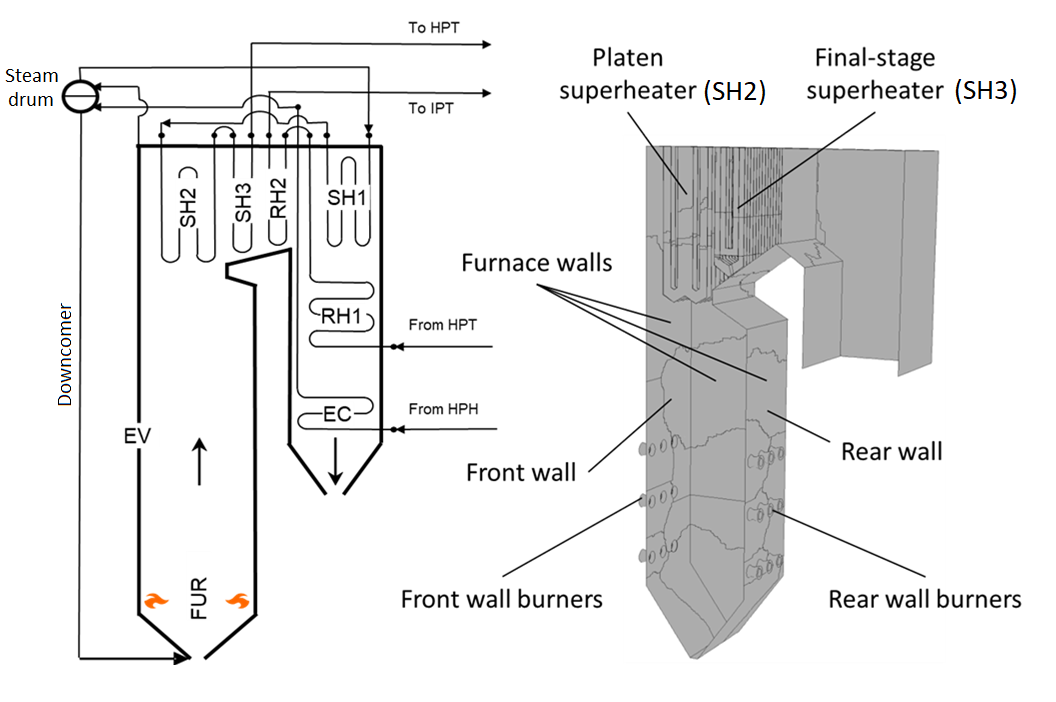
\includegraphics[scale=0.5]{CASE_STUDY_BOILER}
	  \caption{Case study boiler layout \citep{Rousseau2020}.}\label{fig_case_layout}
\end{figure}

The boiler forms part of a 620 MWe power plant and consists of a furnace with water wall evaporator (EV), primary superheater (SH1), platen superheater (SH2) and final superheater (SH3), as well as a primary reheater (RH1), secondary reheater (RH2) and economizer (EC).  The furnace height, width and depth are 64 m, 24 m, and 13.7 m respectively.  The combustion chamber is fitted with three rows of six swirl burners each on the front and rear walls.  Primary air is injected via the inner annulus of the burners, and secondary air via the outer annulus (refer to Figure \ref{fig_cfd_geom_bc}).

\subsection{Integrated model layout}

The validation and the subsequent case-studies presented here, make use of an integrated surrogate and network based 1D process model. The process model is used to capture the thermodynamic response of the water/steam side of the utility boiler under investigation, with the developed data-driven surrogate model providing predictions of the gas-side thermal characteristics (i.e. combustion product species, temperature and incident radiation flux) and heat-exchanger heat loads to the EV, SH2 and SH3 walls.\\

The network model is set up in the process modelling software, Flownex SE\textsuperscript{\textregistered} 2021 \cite{flownex}.  The software can solve both the steady state and transient forms of the fundamental conservation equations of mass, energy, and momentum together with built in fluid property relations and component characteristics representative of all the different types of components.  It is also possible to add control elements to obtain a complete integrated dynamic system simulation model of a plant, sub system or component. 

In the current work a C\# script is used to access the Python application programming interface (API). This allows for predictions to be made using the trained MDN model developed in Python code. The predictions are retrieved using the script and transferred to the respective process model components as inputs. A schematic of the process model and its integration with the surrogate model is provided in Figure \ref{fig_int_model}.\\
\begin{figure}[h!]
	\centering
		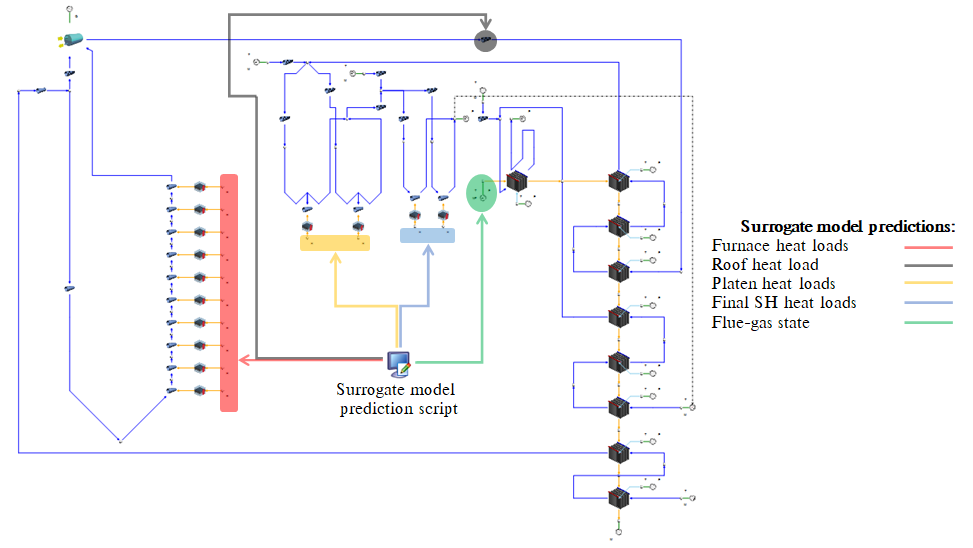
\includegraphics[scale=0.15]{INTEGRATED_MODEL}S
	  \caption{Schematic of network based process model integrated with the surrogate model.}\label{fig_int_model}
\end{figure}

The boiler can be split into three sections namely, the furnace consisting of EV waterwalls, the radiative pass consisting of SH2 and SH3, and the convective pass consisting of RH2, SH1, RH1 and the EC. The furnace heat load predictions to the EV walls determine the evaporation rate. The high pressure (HP) steam outlet flow rate is calculated as the sum of the attemperation flow rates (ATT1 and ATT2) and the evaporation flow rate. The attemperators are used to control the steam temperature to ensure an exit temperature of $808K$ at both the HP outlet and RH outlet. In addition to the furnace heat loads the surrogate model predicts the SH2 and SH3 heat loads. Lastly the surrogate model is able to predict the flue-gas conditions at the inlet to the convective pass (i.e. RH2). The EV, SH2 and SH3 walls are each represented by a single lumped parameter pipe flow component, interconnected with nodes that introduce the attemperation flows to the water/steam side. The convective pass components are modelled using an in-house heat exchanger model that accounts for the radiative (gas and direct), convective and conduction heat transfer mechanisms to and from the gas-side and steam-side control volumes, as well as between the up- and downstream heat exchangers on the gas side.

\section{Applicable machine learning theory}
The present work makes use of various machine learning architectures to develop a surrogate model that can predict the thermal and combustion characteristics of a utility scale boiler using high level inputs. The current section discusses the details of the respective architectures, namely linear regression, ANN and MDN models.
\newpage
\subsection{Multivariate linear regression}
A multivariate linear regression model was established as a base model for comparative purposes in the validation case study of Section \ref{sec_result_1}. The main assumption of a multiple linear regression model is that the output/s can be calculated from a linear combination of the input variables. In other words, a linear regression models aims to determine the quantitative linear relationship between the dependent and independent variables \cite{Wen2022}. The representation of the $i$-th dependent variable ($y_i$) can be written as follows for $m$-number of independent variables ($x_{mi}$);
\begin{equation}
\begin{split}
&y_i = \beta_0+\beta_1 x_{1i}+...+\beta_m x_{mi}\\
&i = 1,2,3...n
\end{split}
\end{equation}
where $\beta_0$ is a constant term, $\beta_{m}$ is the $m$-th coefficient, and $n$ is the total number of observations.\\
 
The optimal solution can be estimated by minimizing the cost function ($J$). A cost function usually calculates the difference between the estimated and the desired values and is reported as a single number. Multivariate linear regression problems typically utilize the mean square error (MSE) between the desired and estimated ($\hat{y_i}$)  values \cite{Wheeler2019}, which is given in Equation \ref{eqn_lin_cost}.
 \begin{equation}\label{eqn_lin_cost}
J_{MSE}=\frac{1}{n}\sum^n_{i=1}(y_i-\hat{y_i})^2
\end{equation} 

In the present work we utilised the gradient descent algorithm \cite{Wen2022} to minimize the cost function. The gradient descent algorithm is an iterative procedure used to find the local minimum/maximum. Considering the cost function as a function of the weight, the algorithm can be written as shown in Equation \ref{eqn_grad_descent}.  
\begin{equation}\label{eqn_grad_descent}
\beta_{m} = \beta_m-\eta\frac{\partial}{\partial\beta_m}J(\beta_m)
\end{equation}
where $\eta$ is known as the learning rate.\\

In most cases the relationship between the dependent and independent variables are not linear. Special non-linear basis models, such as polynomial, sinusoidal, and radial can be used to optimize the training results \cite{Rasmussen2006}. For the current work a multiple linear regression model is utilized as a base model for comparison in Section \ref{sec_result_1}. 
\subsection{Multilayer perception networks}
Artificial neural networks (ANN) are machine learning systems inspired by biological neural activity \cite{Rasmussen2006}. There are many classifications of ANNs, with multilayer perception networks (MLP) being the standard representation \citep{goodfellow}. Typically, MLPs are adapted for supervised learning problems where the input variables are mapped to labelled output variables. The relationship between the input and output variables are learned by optimizing the weights ($\overline{w}$) and biases ($\overline{b}$) to minimize a selected cost function, which for most cases is the MSE given in equation \ref{eqn_lin_cost}. A standard MLP schematic is given in figure \ref{fig_mlp_schematic}, illustrating the common features of a MLP, that being the input, hidden and output layers.\\

To calculate the output values ($\hat{y_i}$) the forward propagation algorithm is utilized, which calculates the output for each layer and moves sequentially through the network until an output is determined. Each network layer output is calculated using two steps, the first being the calculation of the summed signal $\overline{z}_l$ and secondly the use of an activation function to generate the output signal $\overline{h}_l$. Equation \ref{eqn_summed_sig} highlights the first step, where $\overline{h}_{l-1}$ is the output signal from the previous layer.
\begin{equation}\label{eqn_summed_sig}
\overline{z}_l = \overline{h}_{l-1}\cdot\overline{w}_l+\overline{b}_l
\end{equation}

The result of equation \ref{eqn_summed_sig} is subsequently passed to an activation function ($\overline{h}_l = \sigma_l(\overline{z}_l)$). There are various activation functions that can be utilized, such as linear, ReLu, Elu, and the hyperbolic tangent \citep{goodfellow}, with the final layer activation function usually being linear for regression models. The current work makes use of ReLu for the hidden layers, since the ReLu are simple to implement and fast to compute \cite{Wheeler2019}, and a linear activation function for the output layer/s. The ReLu and linear activation functions are shown in Equation \ref{eqn_act_func}.
\begin{figure}[h!]
	\centering
		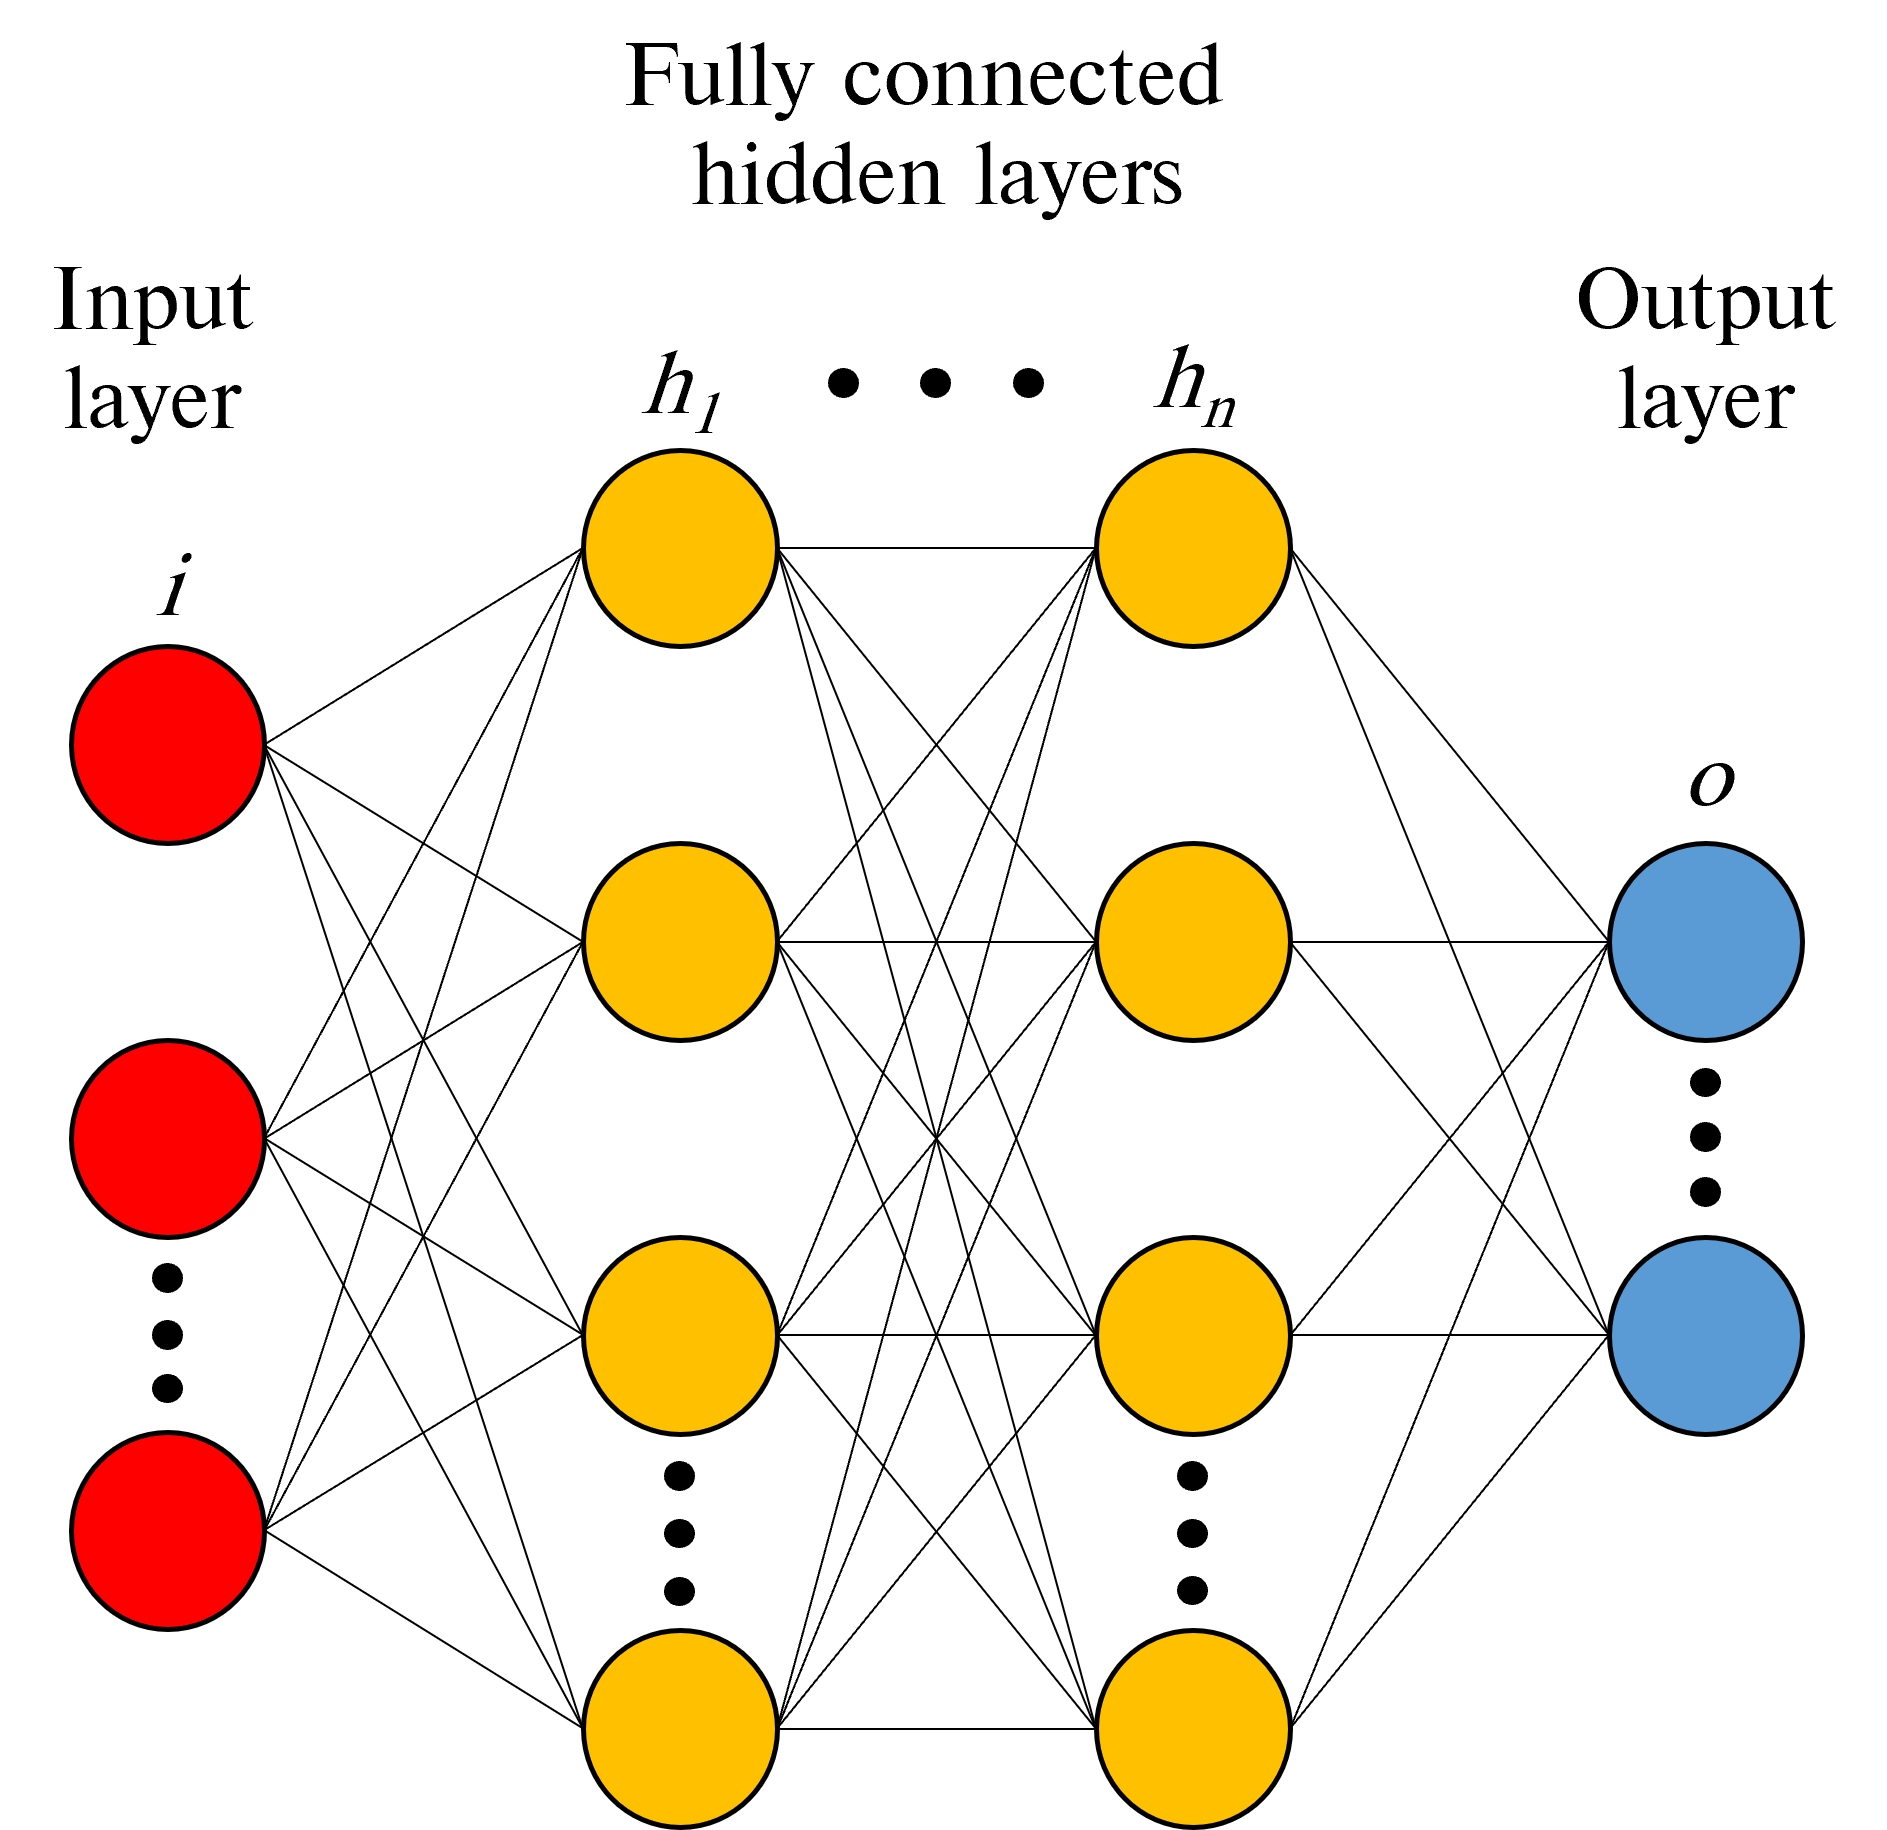
\includegraphics[scale=0.5]{ML_SCHEMATIC}
	  \caption{Traditional MLP schematic.}\label{fig_mlp_schematic}
\end{figure}
\begin{equation}\label{eqn_act_func}
\begin{split}
&\overline{h}_l=\sigma_{ReLu}(\overline{z}_l) = \overline{z}_l =  
	\begin{cases}
	 \overline{h}_{l-1}\cdot\overline{w}_l+\overline{b}_l\,\, &if\,\,\,\, \overline{z}_l>0\\
	 0\,\, &if\,\,\,\, \overline{z}_l<0
	\end{cases}\\
&\overline{h}_l=\sigma_{linear}(\overline{z}_l) = \overline{z}_l = \overline{h}_{l-1}\cdot\overline{w}_l+\overline{b}_l
\end{split}
\end{equation}

When the forward propagation step is complete, the network weights and biases can be updated to minimize the cost function (refer to Equation \ref{eqn_lin_cost}) using the backward propagation method \cite{Rumelhart1986}. The methodology calculates the gradient of the cost function with respect to the weights and biases for each layer. Once the gradients have been calculated the weights and biases are updated using the gradient descent algorithm. The current work makes use of the Adam \cite{goodfellow} alternative to the gradient descent algorithm, which is illustrated in Equation \ref{eqn_adam_algor}. Forward- and backward-propagation algorithms would be iteratively conducted until the cost function is reduced to below a desired threshold.
\begin{theorem} 
\begin{equation}\label{eqn_adam_algor} 
\begin{split}
&\overline{m}\leftarrow \beta_1\overline{m}+(1-\beta_1)\nabla_{\theta}J_{MSE}(\overline{\theta})\\
&\overline{s}\leftarrow \beta_1\overline{s}+(1-\beta_2)\nabla_{\theta}J_{MSE}(\overline{\theta})\otimes&\nabla_{\theta}J_{MSE}(\overline{\theta})\\
&\overline{m}\leftarrow\frac{\overline{m}}{1-\beta_1^t} \\
&\overline{s}\leftarrow\frac{\overline{s}}{1-\beta_2^t}\\
&\overline{\theta}\leftarrow\overline{\theta}-\eta\overline{m}\otimes(\sqrt{\overline{s}+\epsilon})^{-1}\\
\end{split}
\end{equation}
\end{theorem}

The variable $\bar{\theta}$ in Equation \ref{eqn_adam_algor} represents the model weights and biases for each layer. Scaling ($\bar{s}$) and the momentum ($\bar{m}$) matrices are initialized to zero when beginning the training phase. $t$ is the iteration counter, while $\beta_1$ and $\beta_2$ are the momentum and scaling decay hyper-parameters set to values of 0.9 and 0.999 respectively. Lastly $\epsilon$ is a smoothing term set to a value of $10^{-8}$. In the present work various learning rates ($\nu$) were investigated during the hyper-parameter search for both the MLP and MDN neural architectures.

\subsection{Mixture density networks (MDNs)}
Mixture density networks are fundamentally built from two components, namely an ANN and a mixture model. This allows for multi-modal predictions. The ANN can be a standard feed-forward MLP or a recurrent neural network (RNN), with RNNs being used in transient applications with at least one feedback loop \citep{Oko2015}.\\

MDNs are used to predict the parameters of a probability distribution ($P(\overline{X}\mid\overline{Y})$), allowing for non-Gaussian distributions to be modelled, thus making MDNs a probabilistic machine learning framework. MDNs estimate the conditional probability distribution as a mixture of Gaussian distributions where the mixing coefficients ($\overline{\pi}_k$) and component densities are flexible functions of the input data ($\overline{X}$). Equation \ref{eqn_cond_prob_func} illustrates the conditional probability function.
\begin{equation}\label{eqn_cond_prob_func}
P(\overline{X}\mid\overline{Y}) = \sum_{k=1}^K\overline{\pi}_k(\overline{X})\cdot \mathbb{N}(\overline{Y}\mid \overline{\mu}_k(\overline{X}),\overline{\sigma}^2_k(\overline{X}))
\end{equation}
where $K$ represents the number of selected normal distributions, while $\overline{\mu}_k$ and $\overline{\sigma}^2_k$ are the predicted means and variances for each distribution $k$ given the input data $\overline{X}$ respectively.\\

A schematic of a simple MDN network is given in Figure \ref{fig_mdn_schematic}, highlighting the mixing coefficients, predicted means and deviations. It is shown that modifications are made to the output layer by splitting the network output into three parts to calculate the $\overline{\pi}_k$, $\overline{\mu}_k$ and $\overline{\sigma}^2_k$ for each $k$ distribution. This enables the MDN network to learn the $P(\overline{X}\mid\overline{Y})$.\\
\begin{figure}[h!]
	\centering
		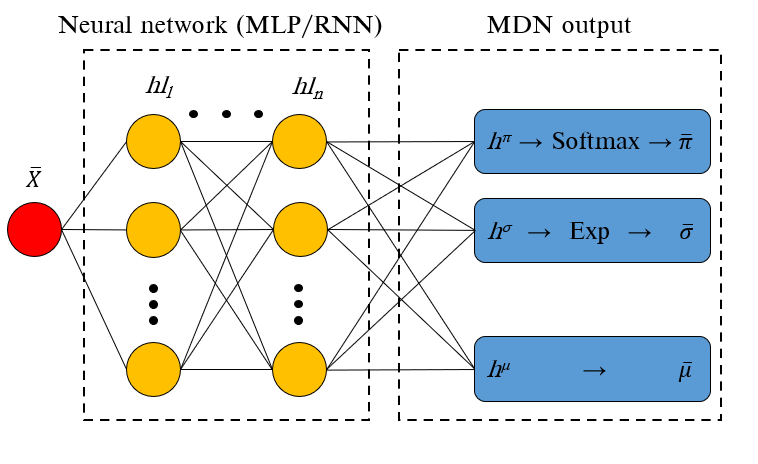
\includegraphics[scale=0.5]{MDN_SCHEMATIC}
	  \caption{Simple MDN network.}\label{fig_mdn_schematic}
\end{figure}

Bishop \cite{bishop1994} proposed the following restrictions for the mixing coefficients and variance components of the MDN output layer. Since the mixing coefficients contain the discrete probabilities of an output belonging to each $K$ normal distribution for all observations, the mixing coefficients must satisfy the constraints listed in Equation \ref{eqn_mix_coef_constraint}.
\begin{equation}\label{eqn_mix_coef_constraint}
\begin{split}
&\sum_{k=1}^K\overline{\pi}_k^n=1\\
&0\leq\overline{\pi}_k^n\leq1
\end{split}
\end{equation}
These constraints are met by using a Softmax function on the output of the hidden layer $h^{\pi}$. The mixing coefficient is calculated using Equation \ref{eqn_mix_coeff}.
\begin{equation}\label{eqn_mix_coeff}
\overline{\pi}_k^n(\overline{x}^n)=\frac{exp(h_k^{\pi,n})}{\sum_{k=1}^Kexp(h_k^{\pi,n})}
\end{equation}

Similarly, a constraint is applied to the standard deviation values ensuring a positive value, this is achieved using an exponential function being applied to the standard deviation leg of the MDN output layer, namely $h^{\sigma}$. Equations \ref{eqn_stddev} shows the imposed constraint for the standard deviation leg.\\
\begin{equation}\label{eqn_stddev}
\begin{split}
&(\overline{\sigma}^n_k(\overline{x}^n))^2\geq 0\\
&\sigma_k^n(\overline{x}^n)=exp(h_k^{\sigma,n})
\end{split}
\end{equation}

The MDN weights and biases are optimized by minimizing the negative log-likelihood for all observations in a batch. This is shown in Equation \ref{eqn_nll}.
\begin{equation}\label{eqn_nll}
J_{NLL}(\overline{Y},\overline{\pi},\overline{\sigma},\overline{\mu})=-\sum^N_{n=1}ln\left\{\sum^K_{k=1}\overline{\pi}_k(\overline{X}^n,\overline{\theta})\cdot \mathbb{N}(\overline{Y}^n\mid\overline{\mu}_k(\bar{X}^n,\bar{\theta}),\overline{\sigma}^2_k(\overline{X}^n,\overline{\theta})) \right\}
\end{equation}
\section{Data generation}
A steady-state multiphase non-thermal equilibrium CFD model was used to generate the training and testing data, which was subsequently used for training/testing of an appropriate surrogate model.
\subsection{CFD model setup}
The current study makes use of an existing steady-state multiphase CFD model \cite{Rawlins2021, INFUB2022} of the boiler under investigation using the commercial CFD software package ANSYS\textsuperscript{\textregistered} Fluent 2019 R3 to resolve the fluid flow, heat transfer and combustion processes. This section provides a short overview of the model for the sake of completeness.\\

The modelled boiler consisted of a furnace with a depth of 13.77 ($m$), width of 24.01 ($m$) and maximum height of 64.00 ($m$). The CFD computation domain was created for half of the furnace width and has a symmetry boundary condition loacted at 12.01 ($m$). This was done to reduce the total cell count of the numerical mesh. Figure \ref{fig_cfd_geom_bc} highlights the computational domain and defines the important boundary conditions. The general conservation equations of mass, momentum, energy, and species were solved using a Eulerian approach. These are provided in Equation (\ref{eqn_cfd}).
\begin{figure}[h!]
	\centering
		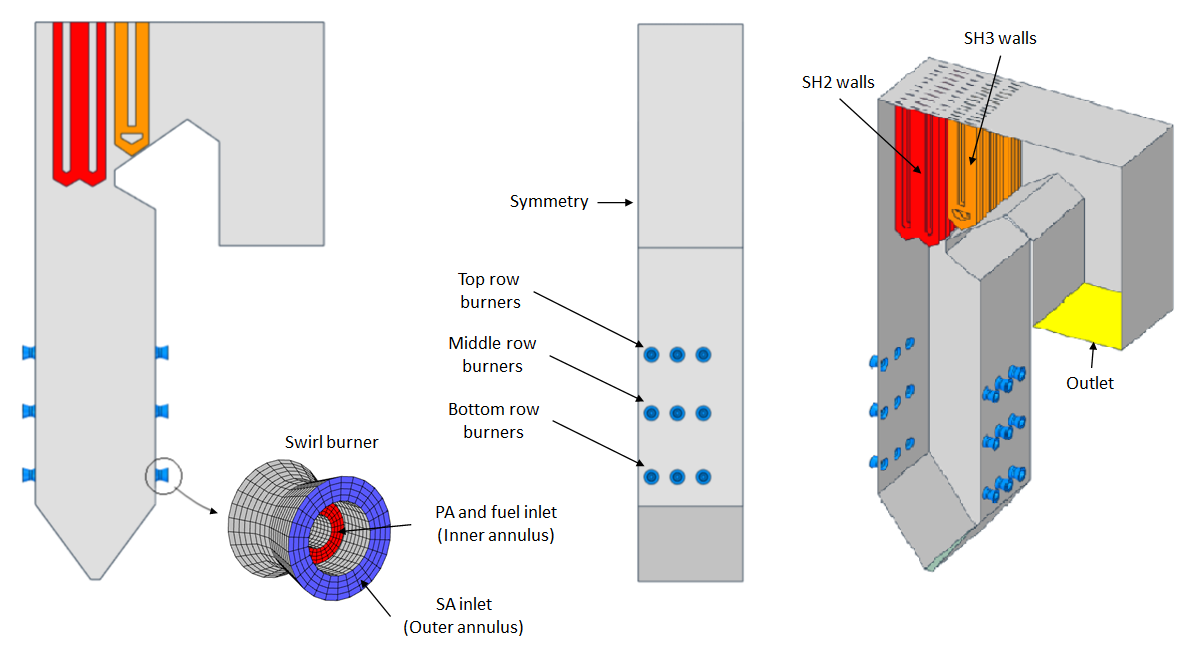
\includegraphics[scale=0.45]{CFD_GEOMETRY}
	  \caption{CFD model geometry and boundary condition descriptions.}\label{fig_cfd_geom_bc}
\end{figure}
\begin{flalign} \label{eqn_cfd}
&\frac{\partial}{\partial x_{i}}(\rho \bar{u}_{i})=S \nonumber &&\\
&\frac{\partial}{\partial x_{i}}(\rho_{eff} u_{i}u_{j})+\frac{\partial \overline{p}}{\partial x_{j}}= \nonumber&&\\
&\frac{\partial}{\partial x_{i}}\left[\mu\left\{\frac{\partial u_{j}}{\partial x_{i}}+\frac{\partial u_{i}}{\partial x_{j}}-\frac{2}{3}\delta_{ij}\frac{\partial u_{i}}{\partial x_{i}}\right\}\right]+\frac{\partial}{\partial x_{i}}(-\rho\overline{u_{i}^{'}u_{j}^{'}})+S_m \nonumber \nonumber &&\\
&\frac{\partial }{\partial x_{i}} (u_{i}[\rho E+p])=\frac{\partial }{\partial x_{j}}\left[\lambda\frac{\partial T_{g}}{\partial x_{j}}\right] +S_{h} &&\\
&\frac{\partial}{\partial x_{i}}(\rho u_{j}Y_{k})=-\frac{\partial}{\partial x_{j}}(\vec{J_{k}})+ \sum_r R_{j,r} + S_{k} \nonumber && 
\end{flalign}

The solution of the Reynolds stress term found in the momentum equation ($-\rho\overline{u_{i}^{'}u_{j}^{'}}$) was approximated using the Boussineq equation \citep{Versteeg2007}. In the present study the realizable k-$\varepsilon$ turbulence model was utilized to address the turbulence closure problem and was selected for its applicability in modelling the effects of coal-fired swirl burners \citep{Modlinski2010}.\\

The P1 radiation model was used to resolve the radiative field in the domain. Particle transport was modelled using a multiphase Eulerian-Eulerian approach, further details of which are provided in the validation study of Rawlins et al \citep{Rawlins2021, Rawlins2022}. Modelling of combustion follows a four-step sequential process, beginning with the heating and evaporation of the moisture present in the fuel, followed by the devolatilization process where the volatiles are liberated from the solid particle, followed by the phenomena of char burnout, and finally the gas phase reactions would commence. The char oxidation reaction product species was set to that of carbon monoxide ($CO$). For the gas-phase reactions the turbulence-chemistry interaction was approximated using the eddy dissipation model (EDM). A summary of the combustion equations and constants is provided in Table \ref{tbl_combust}.\\
\begin{table}[h!]
\caption{Summary of combustion models and constants used in the CFD model}\label{tbl_combust}
\begin{tabular*}{\tblwidth}{p{0.325\textwidth}p{0.35\textwidth}p{0.25\textwidth}}
\toprule
Model & Equation/s & Constant/s\\
\midrule
\multicolumn{3}{l}{\textit{Devolatilization}} \\ % Table header row
Single rate kinetic model &$\frac{dm_{vol}}{dt} = R_{vol}(m_{0,vol}-m_{vol})$,  & $A_{vol} = 2\times10^5 [s^{-1}]$, \\
& $R_{vol} = A_{vol}exp\left(\frac{E_{a,vol}}{RT_p}\right)$ & $ E_{a,vol} = 6.7\times10^7 [J/kmol]$ - \cite{Sheng2004} \\
\multicolumn{3}{l}{\textit{Char oxidation}} \\
Diffusion/kinetic - \citep{Baum1971} & $\frac{dm_{char}}{dt} = -A_p p_{O_{2}} \frac{R_{diff}R_c}{R_{diff} + R_c}$,  & $A_{c} = 0.0053 [kg/m^2sPa]$, \\
& $R_{c} = A_{c}exp\left(\frac{E_{a,c}}{RT_p}\right)$,  & $E_{a,c} = 8.37\times10^7 [J/kmol]$ - \cite{Sheng2004} \\
& $R_{diff} = \frac{5\times10^{-12}}{d_p} \left(\frac{T_g+T_p}{2}\right)^{0.75}$&\\
\multicolumn{3}{l}{\textit{Gaseous reactions of volatiles and $CO$}} \\
Eddy dissipation model - \cite{Ansys} & $R_{k,r,P} =\vartheta_{k,r}M_{w,k}AB\rho\frac{\varepsilon}{k}min\left(\frac{\sum_{p} Y_p}{\sum_{j}\vartheta_{j,r}M_{w,j}}\right)$, $R_{k,r,R} =\vartheta_{k,r}M_{w,k}A\rho\frac{\varepsilon}{k}min\left(\frac{Y_R}{\vartheta_{R,r}M_{w,R}}\right)$ & $A=4.0$, $B=0.5$\\
\bottomrule
\end{tabular*}
\end{table}

The simulations were solved using the SIMPLE pressure–velocity coupling scheme. The pressure term was discretized using the PRESTO! scheme. Momentum, species, and energy equations were discretized using the second order upwind scheme and the turbulent kinetic energy and dissipation rate using the first-order upwind scheme. The numerical mesh was generated using quadrilateral elements consisting of approximately 6 million cells.  The convergence criteria for the simulation model were set to $1\times10^{-3}$ for the continuity equation, $1\times10^{-4}$ for the velocity equations, $1\times10^{-6}$ for the remaining transport equations, and $1\times10^{-4}$ for monitored key parameters. Convergence criteria was enforced for all the various simulation runs.
\subsection{Simulated dataset}
The inputs to the surrogate model include the following: the excess air ratio per burner, the total mill flowrate for the six mills in operation, the average steam temperatures for the platen and final superheaters, the fouling resistance for the platen and final superheaters, the composition of ash and moisture of the fuel and the gross calorific value of the fuel (which is a function of the fuel composition). Thus the input field has a dimensionality of $d_{inputs}=14$.\\

To obtain a representative set of results for training the surrogate model, a design of experiments (DOE) was conducted to generate a set of 180 simulation cases. The various model input ranges used in the DOE are provided in Table \ref{tbl_doe}. The ranges where selected to cover a wide range of operational loads with maximum continuous ratings (MCR) between 100\% and 30\%. The DOE matrix was populated using the Latin Hypercube Sampling (LHS) method provided in the Python pyDOE library.
\begin{table}[pos =h]
\caption{Design of experiments input ranges for  simulations}\label{tbl_doe}
\begin{tabular*}{\tblwidth}{p{0.5\textwidth}p{0.15\textwidth}p{0.15\textwidth}p{0.15\textwidth}}
\toprule
 Input variables& Min& Max& Units \\ % Table header row
\midrule
 Total fuel flow rate for mills 1 to 6 & 39.5 & 120.2 & $kg/s$ \\
 Fuel proximate analysis moisture mass fraction, $Y_{H_2O}$ & 0.025 & 0.085 & $kg/kg$ \\
 Fuel proximate analysis ash mass fraction, $Y_{ash}$  & 0.259 & 0.559 & $kg/kg$ \\
 Platen SH fouling thermal resistance, $R_{platen}$  & 0.004 & 0.007 & $m^2K/W$ \\
 Final SH fouling thermal resistance, $R_{final}$  &0.01 & 0.017 & $m^2K/W$ \\
\midrule
Input dependent variables& \multicolumn{2}{l}{Function of}& Units\\
\midrule
Higher heating value&\multicolumn{2}{l}{Fuel constituents $Y_{H_2O}$ and $Y_{ash}$}&$J/kg$\\
Excess air & \multicolumn{2}{l}{Total fuel flow rate for mills} & $\%$\\
Platen SH internal steam temperature& \multicolumn{2}{l}{$R_{platen}$} & $K$\\
Final SH internal steam temperature& \multicolumn{2}{l}{$R_{final}$} & $K$\\
\bottomrule
\end{tabular*}
\end{table}

Once the CFD simulations achieved convergence, the target data, comprising of the discretized heat loads to the furnace, platen SH and final SH, the exit flue-gas temperatures and flue-gas composition, was stored for each case. A total of 27 output target values ($d_{targets}$) are extracted from the results for each CFD simulation case. Due to the inherently unsteady nature of the CFD simulations even when convergence has been achieved, the output target values were extracted after every 50 iterations for an additional 2500 iterations once convergence was achieved. This results in each CFD simulation case having a solution data matrix size of ($\bar{Y}\in \mathbb{R}^{50\times27}$).\\

The target dataset was split with 80\% for training purposes and the remainder for testing. To reduce the training time of the neural networks a min-max normalization was utilized to scale all the dataset entries to values between $0\rightarrow1$.
\section{Surrogate model development}
The present work makes use of two types of machine learning models, namely a standard artificial neural network (ANN/MLP) and a mixture density designated model connected to a standard ANN (MDN). The following section will discuss the hyper parameter tuning and final selected model configuration. The programming language Python 3.7.8 and the Tensorflow machine learning libraries were utilized in the present study.
\newpage
\subsection{Model configuration}
The goal of the surrogate model is to predict the heat load distributions to the furnace water walls (EV), the platen superheater (SH2) tubes, and the final superheater (SH3) tubes, as well as the combustion characteristics and flue-gas temperatures at the exit, using the high level inputs for the ranges provided in Table \ref{tbl_doe}.\\

The total CFD solution data matrix size will consist of $180\times\overline{Y}=243000$ data points. Using the total solution data matrix for training and testing would typically result in a slower convergence \cite{goodfellow}. However, the use of subset data packages, referred to as batches or mini-batches, allows for a faster convergence. The batch size is a term used in machine learning that specifies a number of training/testing examples utilized in one iteration \cite{Wheeler2019}. Thus, for a data batch size, $m_b$, the output tensor for the MLP model will be $\hat{Y}\in \mathbb{R}^{m_b\times 27}$ since $d_{targets}=27$. However, the output data for the MDN model will consist of three parts, namely; the mixing coefficients tensor of shape  $\overline{\pi}\in \mathbb{R}^{m_b \times K}$, the output standard deviation tensor of shape $\overline{\sigma}\in \mathbb{R}^{K\times m_b\times 27}$, and the predicted means of tensor shape $\overline{\mu}\in \mathbb{R}^{K\times m_b\times 27}$, where $K$ is the number of distributions. The input data fed into both the MLP and MDN will have shape $\overline{X}\in \mathbb{R}^{m_b\times d_{inputs}}$. The input features will be varied based on the DOE, to account for burner mill biassing, fuel quality and the superheaters fouling thickness.

\subsection{Hyper-parameter tuning \& final model selection}\label{sec_hyper}
Table \ref{tbl_tuning} highlights the hyper-parameter search spaces for both the MLP and MDN model. The MDN has an added parameter, namely the number of additional distributions that the MDN would need to fit to the output data. The hyper-parameter tuning of both the MLP and MDN models made use of 1000 epochs. This was deemed adequate to train/test the models for the various hyper-parameter search spaces and was utilized to reduce the computational effort/time.
\begin{table}[pos=h]
\caption{Hyper-parameter search space for fully connected MLP and MDN models}\label{tbl_tuning}
\begin{tabular*}{\tblwidth}{p{0.5\textwidth}p{0.24\textwidth}p{0.24\textwidth}}
\toprule
 Parameter& MLP search space & MDN search space \\ % Table header row
\midrule
 Number of distributions & - & 1,2,3,4  \\
 Number of layers & 2,3,4 & 2,3,4\\
 Number of neurons per layer & 10, 40, 80, 100  & 10, 40, 80, 100\\
 Learning rates & 1e-3, 1e-4, 1e-5, 1e-6 &  1e-3, 1e-4, 1e-5, 1e-6   \\
 Mini batch sizes  &32, 64, 128, 256 &32, 64, 128, 256  \\
\bottomrule
\end{tabular*}
\end{table}

The hyper-parameter search was conducted in a sequential manner with the MAEs and root mean square errors (RMSE) being taken as important performance indicators for each trained case. Firstly, the hidden layer architecture of both models (MLP \& MDN) were varied by considering the number of hidden layers and neurons per layer. Figure \ref{fig_mlp_hyper} (a) illustrates the MLP model performance for the various hidden layer architectures. The neuron capacity reaches a minimum MAE at 80 neurons per layer for a 4-layer architecture. Further increasing the neuron capacity results in an increase in the MAE, possibly indicating an over fitting of data. Secondly, the learning rates were varied for the best performing architecture of the first hyper-parameter tuning step. Considering Figure \ref{fig_mlp_hyper} (b), a decrease in the learning rate shows an improvement in the MAE, with a learning rate of $1\times10^{-5}$ being the best for the current epoch size. For comparative purposes, learning rates of $1\times10^{-5}$ and $1\times10^{-6}$ were used in the final step, where the mini-batch sizes are varied. Figure \ref{fig_mlp_hyper} (c) highlights the comparison for a fixed epoch, with a mini-batch size of 32 and a corresponding learning rate of $1\times10^{-5}$ showing the best MAE improvement.\\

\begin{figure}[h!]
\centering
    \begin{subfigure}{0.48\textwidth}
    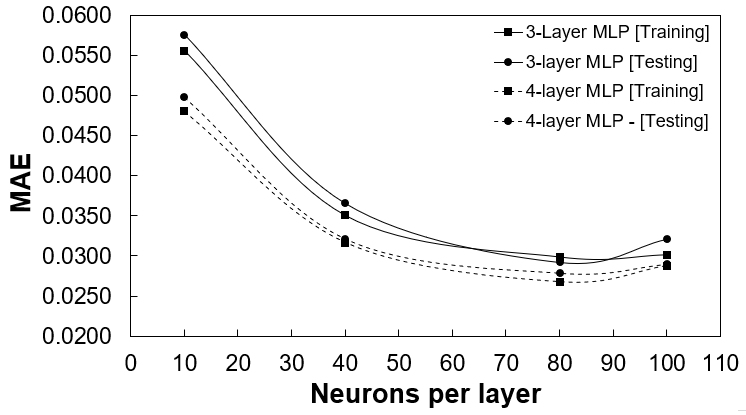
\includegraphics[width=1\textwidth]{NEURONS_HYPER}
    \caption{}
    \end{subfigure}
        \begin{subfigure}{0.48\textwidth}
    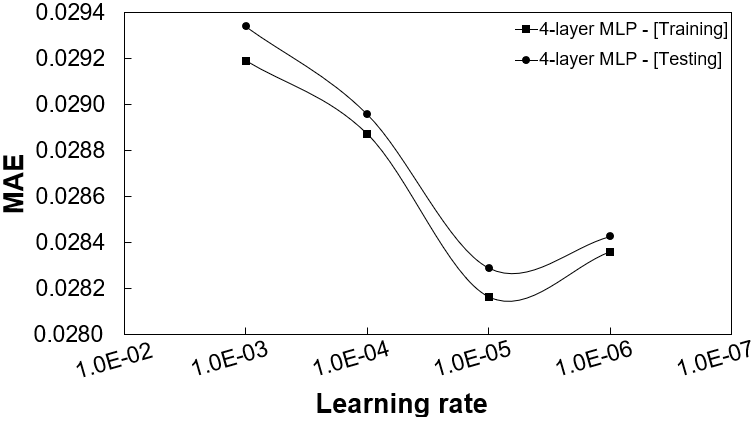
\includegraphics[width=1\textwidth]{LR_HYPER}
    \caption{}
    \end{subfigure}\\
        \begin{subfigure}{0.48\textwidth}
    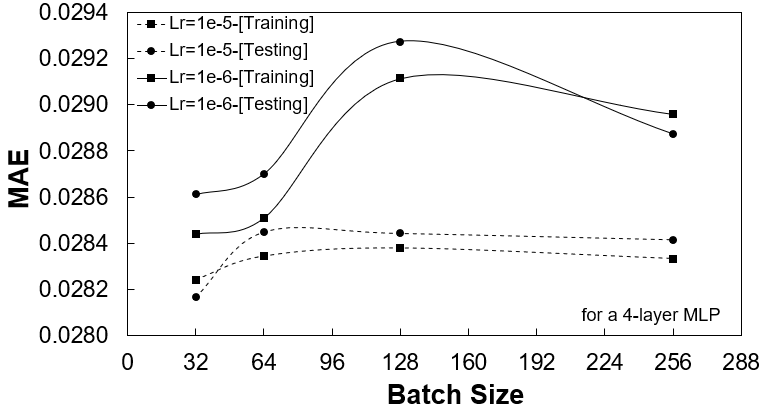
\includegraphics[width=1\textwidth]{BATCH_SIZE_HYPER}
    \caption{}
    \end{subfigure}
    \caption{MLP model performance for; (a) hidden layer architecture, (b) varying learning rates, and (c) varying mini-batch sizes.}\label{fig_mlp_hyper}
\end{figure}

The MDN hyper-parameter tuning was conducted in a similar manner except that an additional step was required. This was to consider the number of distributions the MDN would use to capture the probabilistic characteristics. Figure \ref{fig_mdn_hyper} shows the MAE for the various distributions, with a distribution of one representing the best MLP model. An increase in the number of distributions tends to improve the MAE, however it is evident that a threshold of 3 distributions results in the best improvement.
\newpage
\begin{figure}[h!]
	\centering
		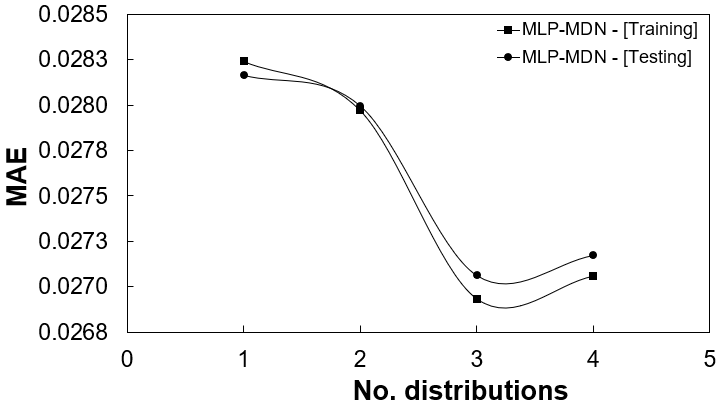
\includegraphics[width=0.48\textwidth]{DIST_HYPER}
	  \caption{MDN model performance for number of distributions.}\label{fig_mdn_hyper}
\end{figure}

The results of hyper-parameter search are given in Table \ref{tbl_hyper_results}. Unlike the MLP, which can only produce a single set of predictions for an input, the MDN is able to produce a distribution of predictions based on the most probable mixing coefficient. This highlights one of the main advantages of the using the MDN model, which is its ability to learn the uncertainty that comes from using a probabilistic model that enables the modelling approach to take into account the effect information density in the training data. This is shown in the error distributions graphs of Figures \ref{fig_frequency_data} (a) and (b). A simple linear regression model was used as a base model for comparative purposes. For the MDN model it is seen that approximately 80-90\% of the training data has mean absolute percentage errors (MAPEs) below 10\%, with the MLP model showing a similar trend. Both models show considerable improvement in comparison to the linear model.\\

\begin{figure}[h!]
\centering
    \begin{subfigure}{0.48\textwidth}
    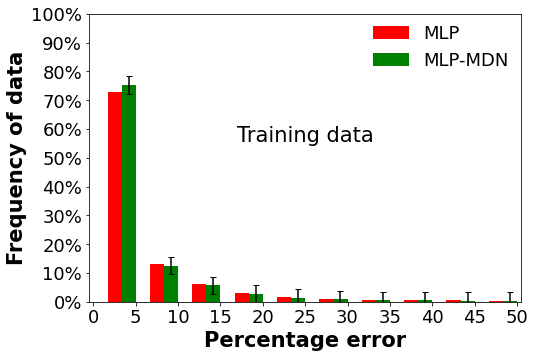
\includegraphics[width=\textwidth]{OVERALL_TRAIN}
    \caption{}
    \end{subfigure}
    \begin{subfigure}{0.48\textwidth}
    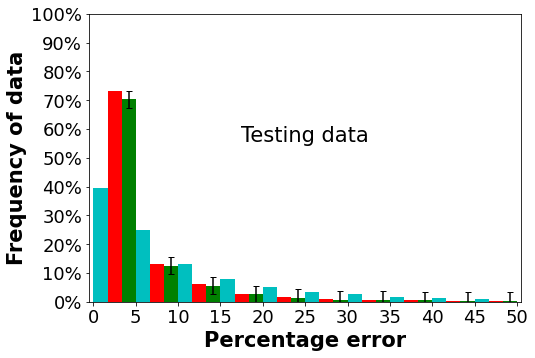
\includegraphics[width=\textwidth]{OVERALL_TEST}
    \caption{}
    \end{subfigure}
    \caption{Error distributions for the selected MLP and MDN model h; (a) training data and (b) testing data.}\label{fig_frequency_data}
\end{figure}

\begin{table}[h!]
\caption{Hyper-parameter search results}\label{tbl_hyper_results}
\begin{tabular*}{\tblwidth}{lp{0.1\textwidth}l}
\toprule
 Parameter& MLP & MDN \\ % Table header row
\midrule
 Number of distributions & - & 3  \\
 Number of layers & 4 & 4\\
 Number of neurons per layer & 80  & 80\\
 Learning rate & 1e-5 &  1e-5   \\
 Mini batch size  &32 & 32  \\
\midrule
Errors & &\\
\midrule
RMSE & 0.0213 & 0.0211\\
MAE & 0.0282& 0.0263\\
\bottomrule
\end{tabular*}
\end{table}  

Based on the above analysis, the MDN model was selected as the best model to be used for the surrogate model implementation. The benefit of using the MDN surrogate model is the ability to provide not only the expected mean (most-probable) value of each output parameter, but also the associated standard deviation. Having the mean value of each of the furnace and heat exchanger heat loads together with its uncertainty in the form of a standard deviation, allows the uncertainty to be propagated through the entire integrated model. It is therefore possible to obtain the resultant mean values of the overall plant performance parameters together with their uncertainties emanating from the surrogate model prediction.

\section{Results and discussion}\label{sec_results_diss}
This section provides the results of the validation study of the integrated model, as well as an application case study that investigates the effects of fuel quality on the integrated boiler performance. 

\subsection{Validation}\label{sec_result_1}
The results predicted using the surrogate model were validated for the 100\%, 80\% and 60\% MCR load cases. Measured data was made available for these load cases, which allow the mean and standard deviation to be determined.  The mean and standard deviation of each output can then be compared with the predicted mean and standard deviation obtained with the integrated model.\\

In the current work the integrated model is applied in conjunction with the Monte Carlo method \cite{Thomopoulos2013}. Firstly, random sampling of the input variables to the integrated model are performed based on the mean and standard deviation predicted by the surrogate model.  Following this, simulations are run for each sample and the outputs are evaluated to determine the predicted mean and standard deviation of each overall plant parameter.\\

Fortunately, Flownex SE\textsuperscript{\textregistered} 2021, provides a built-in Monte Carlo facility. It requires as input the mean and standard deviation values for each model input \cite{flownex}. The Monte Carlo model input used in this study are the predicted mean and standard deviation results obtained with the surrogate model, which utilized the MDN input vectors ($\overline{X}$) provided in Table \ref{tbl_inputs}. These inputs were obtained from the works of Laubscher and Rousseau \cite{Laubscher2019b}. For this study $N=1000$ simulations were performed for each validation case with the mean and standard deviation being used as measures to determine convergence. Table \ref{tbl_fuel_bias} provides the total mill fuel flow rate for the validation cases. Biasing of the mill fuel flow rates was introduced to provide a realistic operational uncertainty to the model.\\

\begin{table}[h!]
\caption{Mill fuel flowrate biasing for the validation case study.}\label{tbl_fuel_bias}
\begin{tabular*}{\tblwidth}{c p{0.1\textwidth}p{0.1\textwidth}p{0.1\textwidth}p{0.1\textwidth}p{0.1\textwidth}p{0.1\textwidth}p{0.1\textwidth}}
\toprule
 MCR load& Mill 1 & Mill 2 &Mill 3 &Mill 4 &Mill 5 &Mill 6 & Unit \\ % Table header row
\midrule
 100\% & 19.14 & 20.22 & 19.92 & 19.98 & 19.41 & 0.00 & $kg/s$  \\
 80\% & 18.23 & 19.72 & 19.02 & 17.82 & 18.02 & 0.00 & $kg/s$  \\
 60\% & 15.46 & 16.13 & 0.00 & 15.11 & 15.32 & 0.00 & $kg/s$  \\
\bottomrule
\end{tabular*}
\end{table}  

\begin{table}[h!]
\caption{MDN input vectors ($\overline{X}$) for the validation and varied fuel case studies}\label{tbl_inputs}
\begin{tabular*}{\tblwidth}{lp{0.12\textwidth}p{0.12\textwidth}p{0.12\textwidth}p{0.12\textwidth}p{0.12\textwidth}}
\toprule
 & \multicolumn{3}{c}{\textbf{Validation load cases}}&\multicolumn{2}{c}{\textbf{Varied fuel load cases}}\\
\textit{Inputs} [\textbf{mean} - ($\overline{\sigma}$)]& 100\%  & 80\% & 60\% & High-ash & High-moisture  \\
\midrule
Excess air ratio - [-] & 1.155 & 1.209 & 1.263 & 1.155 & 1.155  \\
$Y_{ASH}$ - [$kg/kg$] & 0.409 & 0.409 &  0.409 &0.5 & 0.409 \\
$Y_{H_{2}O}$ - [$kg/kg$] & 0.055 & 0.055 & 0.055 & 0.055 & 0.146  \\
HHV = $f(Y_{ASH},Y_{H_{2}O})$ - [$MJ/kg$] & 15.07 & 15.07 & 15.07 & 12.68 & 12.68  \\
Platen SH fouling - [$K/W$]& 0.012 & 0.012 & 0.012 & 0.012 & 0.012  \\
Final SH fouling - [$K/W$] & 0.0067&0.0067 &0.0067 & 0.0067&0.0067  \\
Total fuel flowrate - [$kg/s$] &108.6 & 90.72 & 60.12 &108.6 & 108.6 \\
Platen SH mean steam temp. - [$K$] & 698 &697&781 &698 &698  \\
Final SH mean steam temp. - [$K$]& 787 & 793 &781 &787 &787  \\
\bottomrule
\end{tabular*}
\end{table}  
\begin{figure}
\centering
\begin{subfigure}{0.33\textwidth}
    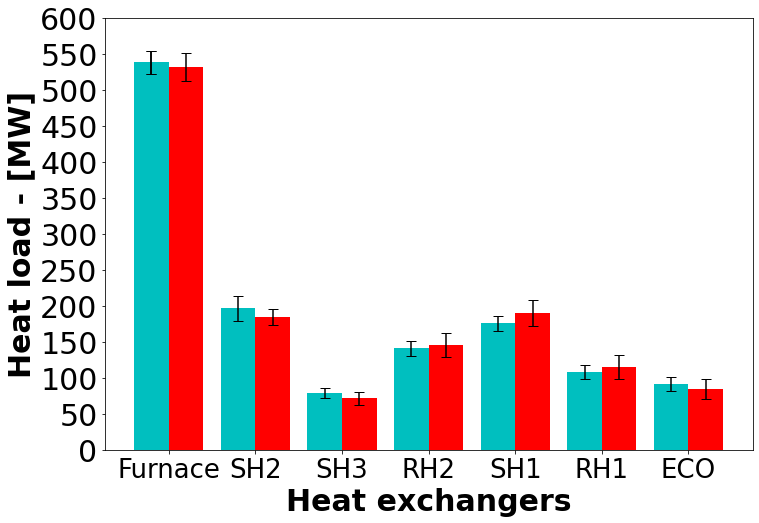
\includegraphics[width=\textwidth, height = 4.25cm]{100_CASE}
    \caption{100\% MCR}
\end{subfigure}\hfill % maximize horizontal separation
\begin{subfigure}{0.33\textwidth}
    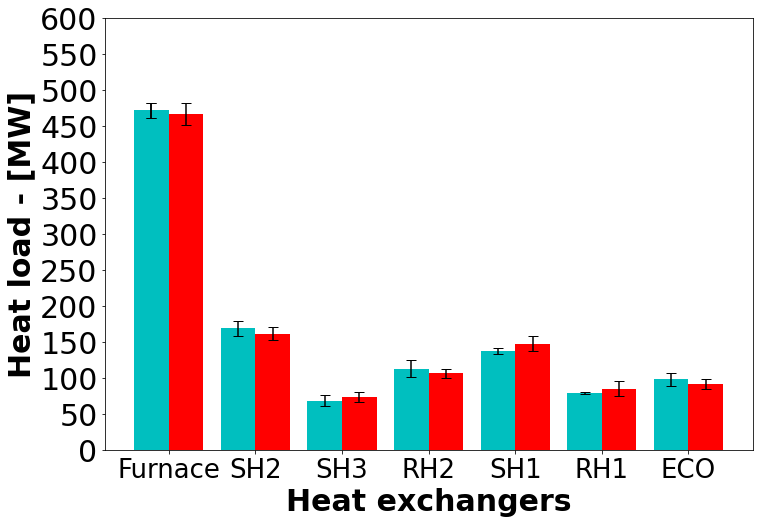
\includegraphics[width=\linewidth, height = 4.25cm]{80_CASE}
    \caption{80\% MCR}
\end{subfigure}\hfill
\begin{subfigure}{0.33\textwidth}
	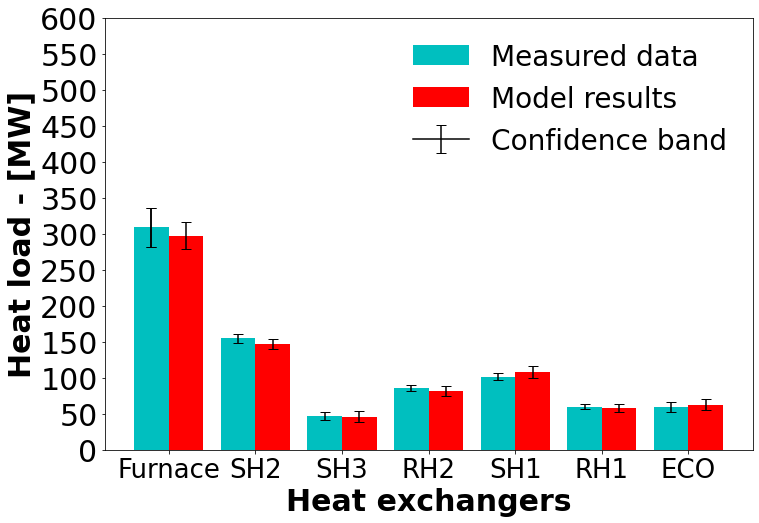
\includegraphics[width=\linewidth, height = 4.25cm]{60_CASE}
        \caption{60\% MCR}
\end{subfigure}
\caption{Load validation result comparison of the measured data and MDN model results for the various heat exchangers}
\label{fig_heat_load}
\end{figure}

\begin{figure}
\centering
\begin{subfigure}{0.33\textwidth}
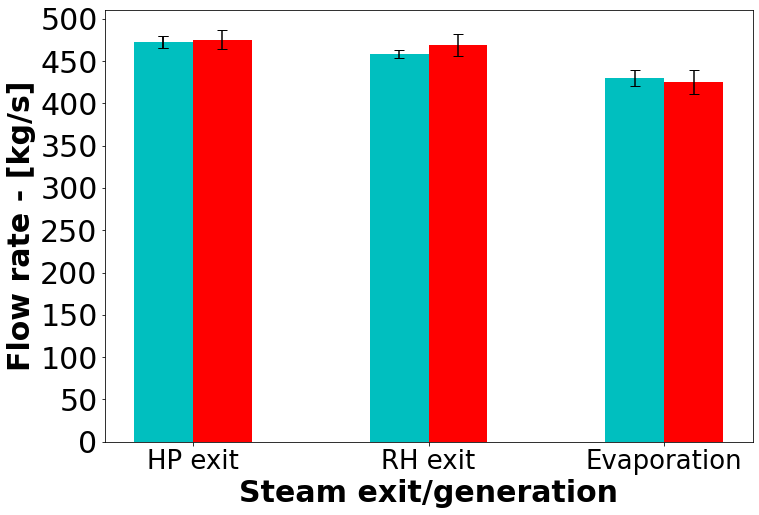
\includegraphics[width=\linewidth, height = 4.25cm]{100_CASE_STEAM}
        \caption{100\% MCR}
\end{subfigure}\hfill % maximize horizontal separation
\begin{subfigure}{0.33\textwidth}
    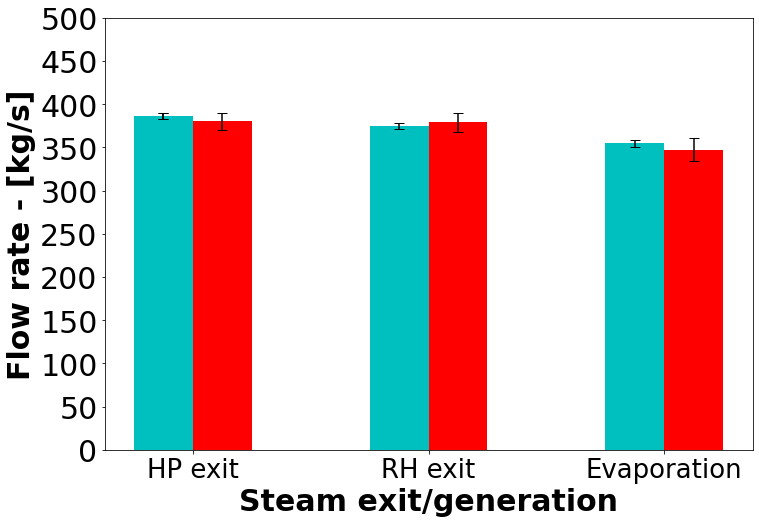
\includegraphics[width=\linewidth, height = 4.25cm]{80_CASE_STEAM}
    \caption{80\% MCR}
\end{subfigure}\hfill
\begin{subfigure}{0.33\textwidth}
	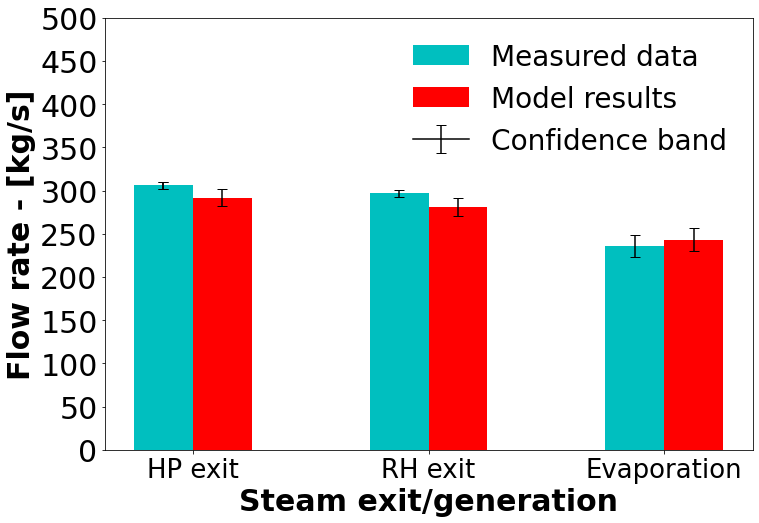
\includegraphics[width=\linewidth, height = 4.25cm]{60_CASE_STEAM}
    \caption{60\% MCR}
\end{subfigure}
\caption{Load validation result comparison of the measured data and MDN model results for the steam exit and  steam generation flowrates}
\label{fig_steam_gen}
\end{figure}

\begin{figure}
\centering
\begin{subfigure}{0.33\textwidth}
    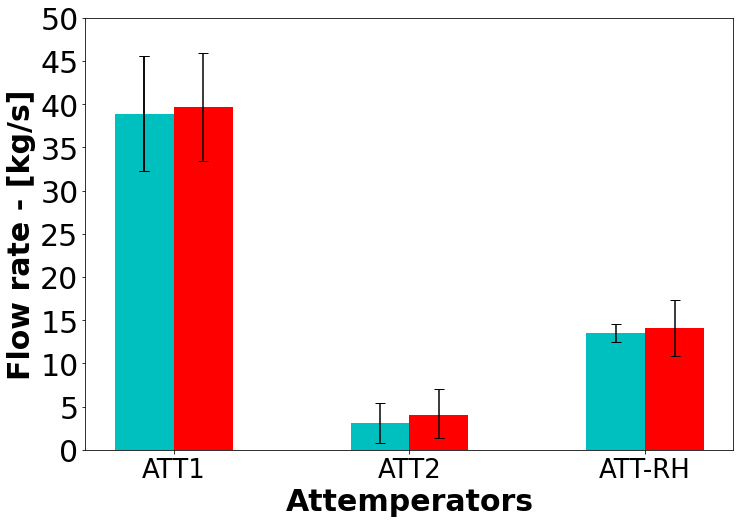
\includegraphics[width=\linewidth, height = 4.25cm]{100_CASE_ATTEMP}
    \caption{100\% MCR}
\end{subfigure}\hfill % maximize horizontal separation
\begin{subfigure}{0.33\textwidth}
    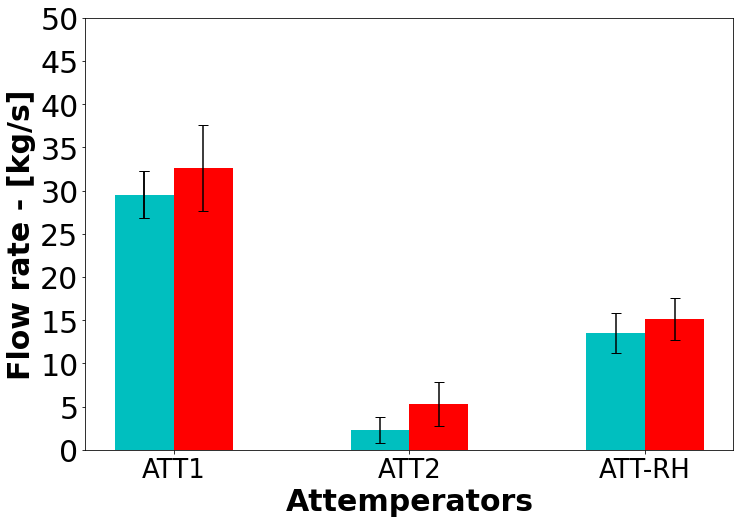
\includegraphics[width=\linewidth, height = 4.25cm]{80_CASE_ATTEMP}
    \caption{80\% MCR}
\end{subfigure}\hfill
\begin{subfigure}{0.33\textwidth}
    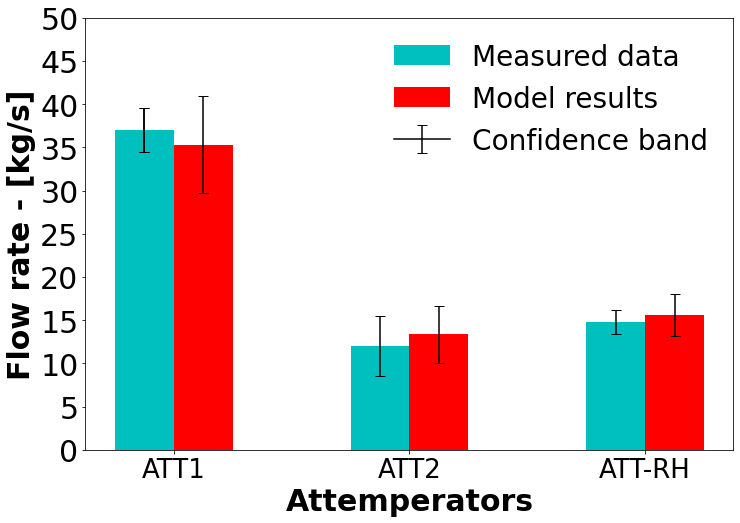
\includegraphics[width=\linewidth, height = 4.25cm]{60_CASE_ATTEMP}
    \caption{60\% MCR}
\end{subfigure}
\caption{Load validation result comparison of the measured data and MDN model results for the required attemperator flowrates to maintain operational integrity}
\label{fig_attemp}
\end{figure}

Figures \ref{fig_heat_load} - \ref{fig_attemp} provide comparative results of the measured data and integrated model responses for all three load cases. It can be seen for a range of MCR loads that the integrated model is able to capture the heat loads to the various heat exchangers (Figures \ref{fig_heat_load} (a-c)) with sufficient accuracy. In general, the model under-predicts the mean of the heat loads in the furnace and radiative pass, with slight over-predictions seen in the convective pass. However, the associated uncertainty of the integrated model overlaps with the measured data uncertainty with minimal outliers, therefore, inferring that the model predictions are sufficiently accurate.\\ 

Considering the steam generation and exit flowrates of Figure \ref{fig_steam_gen} (a-c), the integrated model can sufficiently capture the hydraulic response of the case study boiler for a wide range of loads. More uncertainty is associated with the integrated model, but this is deemed acceptable since the response overlaps with the measured data in all but one case. The attemperators of a utility scale boiler are an integral part of the control systems put in place to ensure safe operating conditions and minimal wear on the downstream components, namely the steam HP and LP steam turbines \cite{Kakac1991}. Figure  \ref{fig_attemp} (a-c) highlight the attemperator flowrates across a wide range of loads. The integrated model is shown to adequately resolve the flowrates with a slightly higher mean being predicted for the 80\% load case.\\

It has been shown that the integrated model is able to resolve the thermal response based on the predictions of the MDN model for a wide range of loads with sufficient accuracy. The heat loads are within a 5\% tolerance of the measured mean values, while the steam generation rates exhibit a maximum difference of 7\%, which is seen in the 60\% MCR load case (refer to Figure \ref{fig_steam_gen} (c)). The attemperator flow rate results show the largest uncertainty/confidence band of all the results (Figure \ref{fig_attemp}), however these overlap with the measured values in all but one case. 
\subsection{Application}
This section demonstrates the application of the validated integrated model by investigating the impact of fuel quality on the overall plant performance. The fuel quality parameters that are varied are the energy content of the fuel ($HHV$), together with the ash ($Y_{ASH}$) and moisture ($Y_{H_{2}O}$) contents. Two case studies are considered to determine the impact of the parameters on the boiler efficiency, heat pick-up and thermal response. The input vectors for the two fuel cases are provided in Table \ref{tbl_inputs}. The inputs are the same as those of the 100\% load case except for the ash, moisture, and higher heating value of the respective fuels.\\

As with the validation case studies of Section \ref{sec_result_1}, the Monte Carlo method was employed to ascertain the mean and standard deviation values predicted via the integrated model. The base case in Figure \ref{fig_fuel_results} (a-c) refers to 100\% load case of Figures \ref{fig_heat_load}-\ref{fig_attemp}. Figure \ref{fig_fuel_results}  (a) highlights the effects that poor quality fuel has on the heat load to the various heat exchangers, with a 20\% drop being observed on average. This can reasonably be expected since the energy content of the fuel is lower than that of the base case. To maintain 100\% load capabilities using the poor quality fuel would require an increase in the fuel flowrate, which would provide more energy content. However, the mill operational capacities are limited. The operational protocol for the 100\% load case makes use of 5 mills operating 30 of the 36 burners at full capacity, with a standby mill and burner arrangement placed in reserve to help mitigate operational risks, such as maintenance schedules. Using the the standby mill would allow the fuel flowrate to be increased by a maximum of 17\%. However, this would in turn decrease the operational integrity and increase the associated risks. This situation would therefore imply an unwanted load loss. When burning the high-ash content fuel the likelihood of ash deposition/fouling of the heat exchanger components also increases.\\

Figure \ref{fig_fuel_results} (b-c) similarly illustrate a decrease in the water/steam flowrates for the steam exit and attemperator conditions. The generation rates exhibit similar characteristics to the the 80\% load case of Figure \ref{fig_steam_gen} (b), illustrating a significant decrease in the operational capabilities when using a poor quality fuel. The predicted flue-gas temperatures entering the the convective pass are shown in Table \ref{tbl_fuel_results}. It is shown that for an increase in the ash content of the fuel, the flue-gas inlet temperature increases, which results in a higher radiative heat transfer percentage for the convective pass components. It is also interesting to note that a higher ash content results in the largest uncertainties in the prediction of the HP and RH exit steam and steam generation flow rates. The presence of more moisture in the fuel results in a lower inlet temperature, primarily due to the fact that the extra moisture requires a higher heat rate of evaporation, leading to lower radiative heat transfer percentages.\\

The boiler efficiency is the measure used to convey how well the combustion heat is transferred to the working fluid, and is defined as the ratio of total amount of heat absorbed by the heat exchangers (i.e. sum of the furnace, radiative and convective pass heat loads) and the combustion energy released ($m_{fuel}HHV$). A significant decrease in the boiler efficiency is highlighted in Table \ref{tbl_fuel_results} for both fuel cases with the high ash fuel showing a slightly better result. The higher efficiency of the high-ash fuel is attributed to the fact that in general the heat loads to various heat exchangers are higher than that of the high-moisture fuel, which can be seen in Figure \ref{fig_fuel_results} (a). 

\begin{table}[h!]
\caption{Model results for poor quality fuel characteristics}\label{tbl_fuel_results}
\begin{tabular*}{\tblwidth}{p{0.3\textwidth}p{0.22\textwidth}p{0.22\textwidth}p{0.22\textwidth}}
\toprule
\textit{Variable} (\textbf{mean}  (\textit{min},\textit{max}))& Base & High-ash & High-moisture \\ % Table header row
\midrule
Mean boiler efficiency [\%]& \textbf{88.2}  (\textit{75.6},\textit{91.2}) & \textbf{77.6}  (\textit{73.4},\textit{80.9}) & \textbf{75.9}  (\textit{69.8},\textit{78.3})\\
Convective pass inlet flue-gas temp. [$K$]& \textbf{1352}  (\textit{1339},\textit{1370}) & \textbf{1368}  (\textit{1354},\textit{1378}) & \textbf{1311}  (\textit{1295},\textit{1327})\\
\midrule
\multicolumn{4}{l}{\textit{Radiative heat transfer percentage (Convective pass)} }\\
\midrule
RH2 & \textbf{52.3}  (\textit{50.1},\textit{54.0}& \textbf{56.2}  (\textit{52.9},\textit{58.5} & \textbf{50.3}  (\textit{47.8},\textit{53.9}\\
SH1 & \textbf{46.3}  (\textit{43.0},\textit{49.2})& \textbf{49.8}  (\textit{44.8},\textit{52.3}& \textbf{47.2} - (\textit{43.2},\textit{50.8}\\
RH1 & \textbf{21.3}  (\textit{16.1},\textit{24.6})& \textbf{26.7}  (\textit{20.6},\textit{30.1}& \textbf{18.2}  (\textit{13.7},\textit{23.5}\\
ECO & \textbf{6.7}  (\textit{5.1},\textit{9.8})& \textbf{8.3}  (\textit{6.3},\textit{12.6}& \textbf{5.4} - (\textit{2.8},\textit{9.7}\\
\bottomrule
\end{tabular*}
\end{table}  

\begin{figure}
\centering
\begin{subfigure}{0.33\textwidth}
    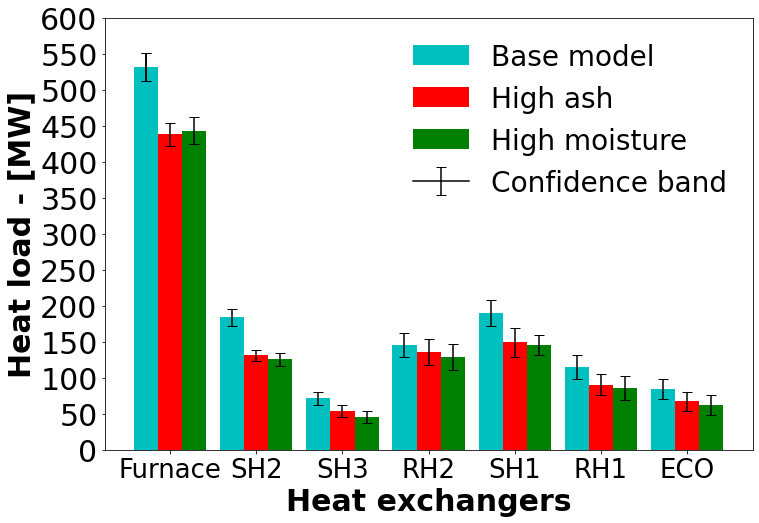
\includegraphics[width=\textwidth, height = 4.25cm]{100_FUEL_CASE}
    \caption{}
\end{subfigure}\hfill % maximize horizontal separation
\begin{subfigure}{0.33\textwidth}
    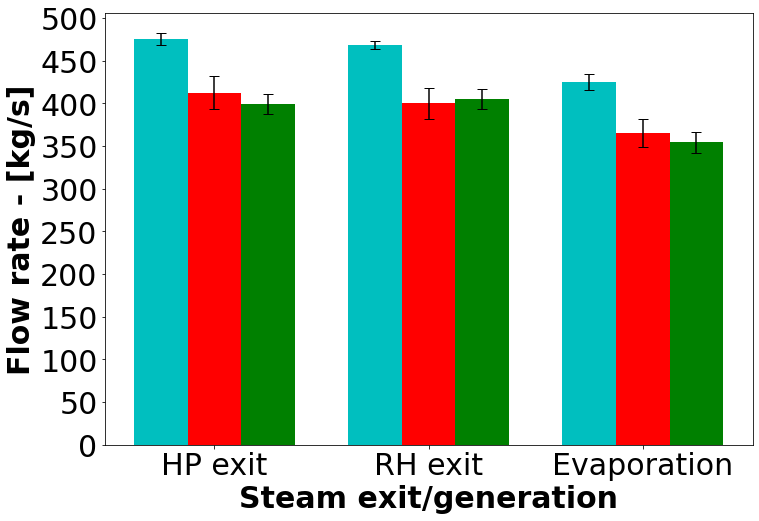
\includegraphics[width=\linewidth, height = 4.25cm]{100_FUEL_CASE_STEAM}
    \caption{}
\end{subfigure}\hfill
\begin{subfigure}{0.33\textwidth}
    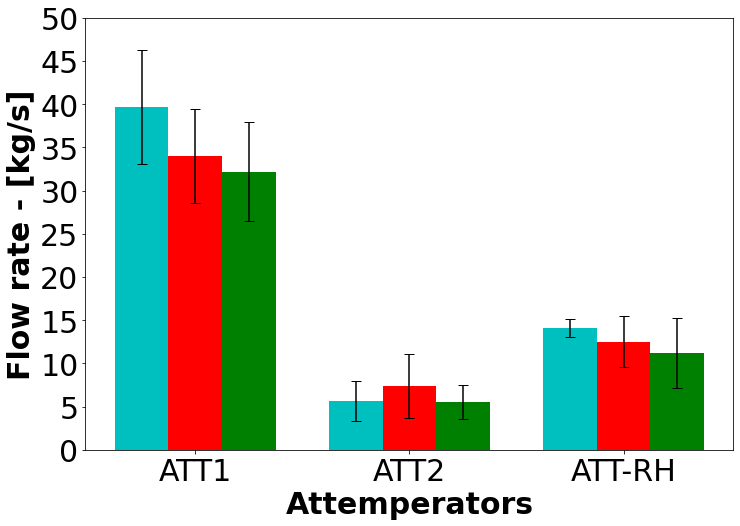
\includegraphics[width=\linewidth, height = 4.25cm]{100_FUEL_CASE_ATTEMP}
    \caption{}
\end{subfigure}
\caption{Integrated base case, high-ash and high-moisture case study comparison for; (a) the various heat exchangers, (b) the steam exit and generation flowrates, and (c) the required attemperator flowrates to maintain operational integrity}
\label{fig_fuel_results}
\end{figure}
\newpage
\section{Conclusion}
The present work establishes the basis for utilizing an integrated data-driven surrogate and 1D process model to investigate the overall operational response for a 620 $MW_e$ utility scale boiler.\\

The data-driven surrogate modelling approach using CFD simulations can predict the various parameters needed to capture the combustion and heat transfer characteristics. These include the heat loads to the furnace evaporator walls (EV) and radiative superheaters (SH2 and SH3), as well as the flue-gas characteristics entering the convective pass, which include the temperatures, species mass fractions and radiation intensity. Training and testing datasets were generated using the CFD model of the 620 MWe. A total of 180 different CFD simulation cases were performed, where the input variables of Table \ref{tbl_doe} were varied.\\

It was found that the best surrogate model architecture was the use of a MDN configuration, which also allows prediction of the associated uncertainties. The configuration comprised of a MDN network consisting of 4 hidden layers each consisting of 80 neurons and 3 normal output distributions, while using a learning rate of $1\times10^{-5}$ and batch size of 32. The MDN network illustrated that approximately 80-85\% of the model predictions had MAPEs below 10\%.\\

A validation case study was performed using the integrated model for a wide range of operational loads. The model results were compared to the measured thermal response for all load cases. The resolution of the heat loads, steam flowrates and attemperation flowrates resulted in a maximum difference of 7\%. The uncertainties predicted by the surrogate model were propagated through the integrated model using the Monte Carlo technique, adding valuable insight into the operational limits of the power plant and the uncertainties associated with it.\\

The application case studies considered the impact of poor quality fuels at 100\% MCR operation. The results highlight the drop in performance due to the fuel quality resulting in a substantial decrease in boiler efficiency. Using a high-ash fuel can result in a higher exit flue-gas temperatures resulting in a marginal increase in performance of the convective pass heat exchangers when compared to the high moisture fuel. However, it results in greater uncertainty in the predicted steam exit and generation flow rates and increases the likelihood of ash deposition occurring.\\ 

The current work has shown that it is possible to adequately resolve the thermofluid response of a utility scale boiler using a data-driven surrogate model trained on CFD simulation results. The integration of the surrogate and 1-D process model is paramount in modelling the thermal response and provides valuable operational insight for various load cases, including the uncertainty in the predicted results. The methodology used in the present work can be applied by engineers and other researchers to investigate various effects on the whole boiler operation.
\printcredits
%% Loading bibliography style file
%\bibliographystyle{model1-num-names}
%\bibliographystyle{cas-model2-names}
\bibliographystyle{elsarticle-num}

% Loading bibliography database
\bibliography{ML_paper}


\end{document}


